\chapter{IBM BigFix}

\section{BigFix}
I prodotti della suite IBM BigFix consentono di monitorare e gestire in tempo reale un elevato numero di dispositivi connessi (fino a 250.000). Questi possono essere sia fisici che virtuali, come ad esempio server, desktop, notebook, dispositivi mobili, tablet, POS, ATM e chioschi self-service. Gli utenti principali di questi prodotti sono gli amministratori di sistema. Tramite le applicazioni BigFix possono avere il pieno controllo sugli endpoint. Possono ad esempio distribuire software, applicare delle patch, effettuare il deploy di sistemi operativi, proteggere da attacchi di rete e molto altro.
\begin{figure}[h!]
	\centering
	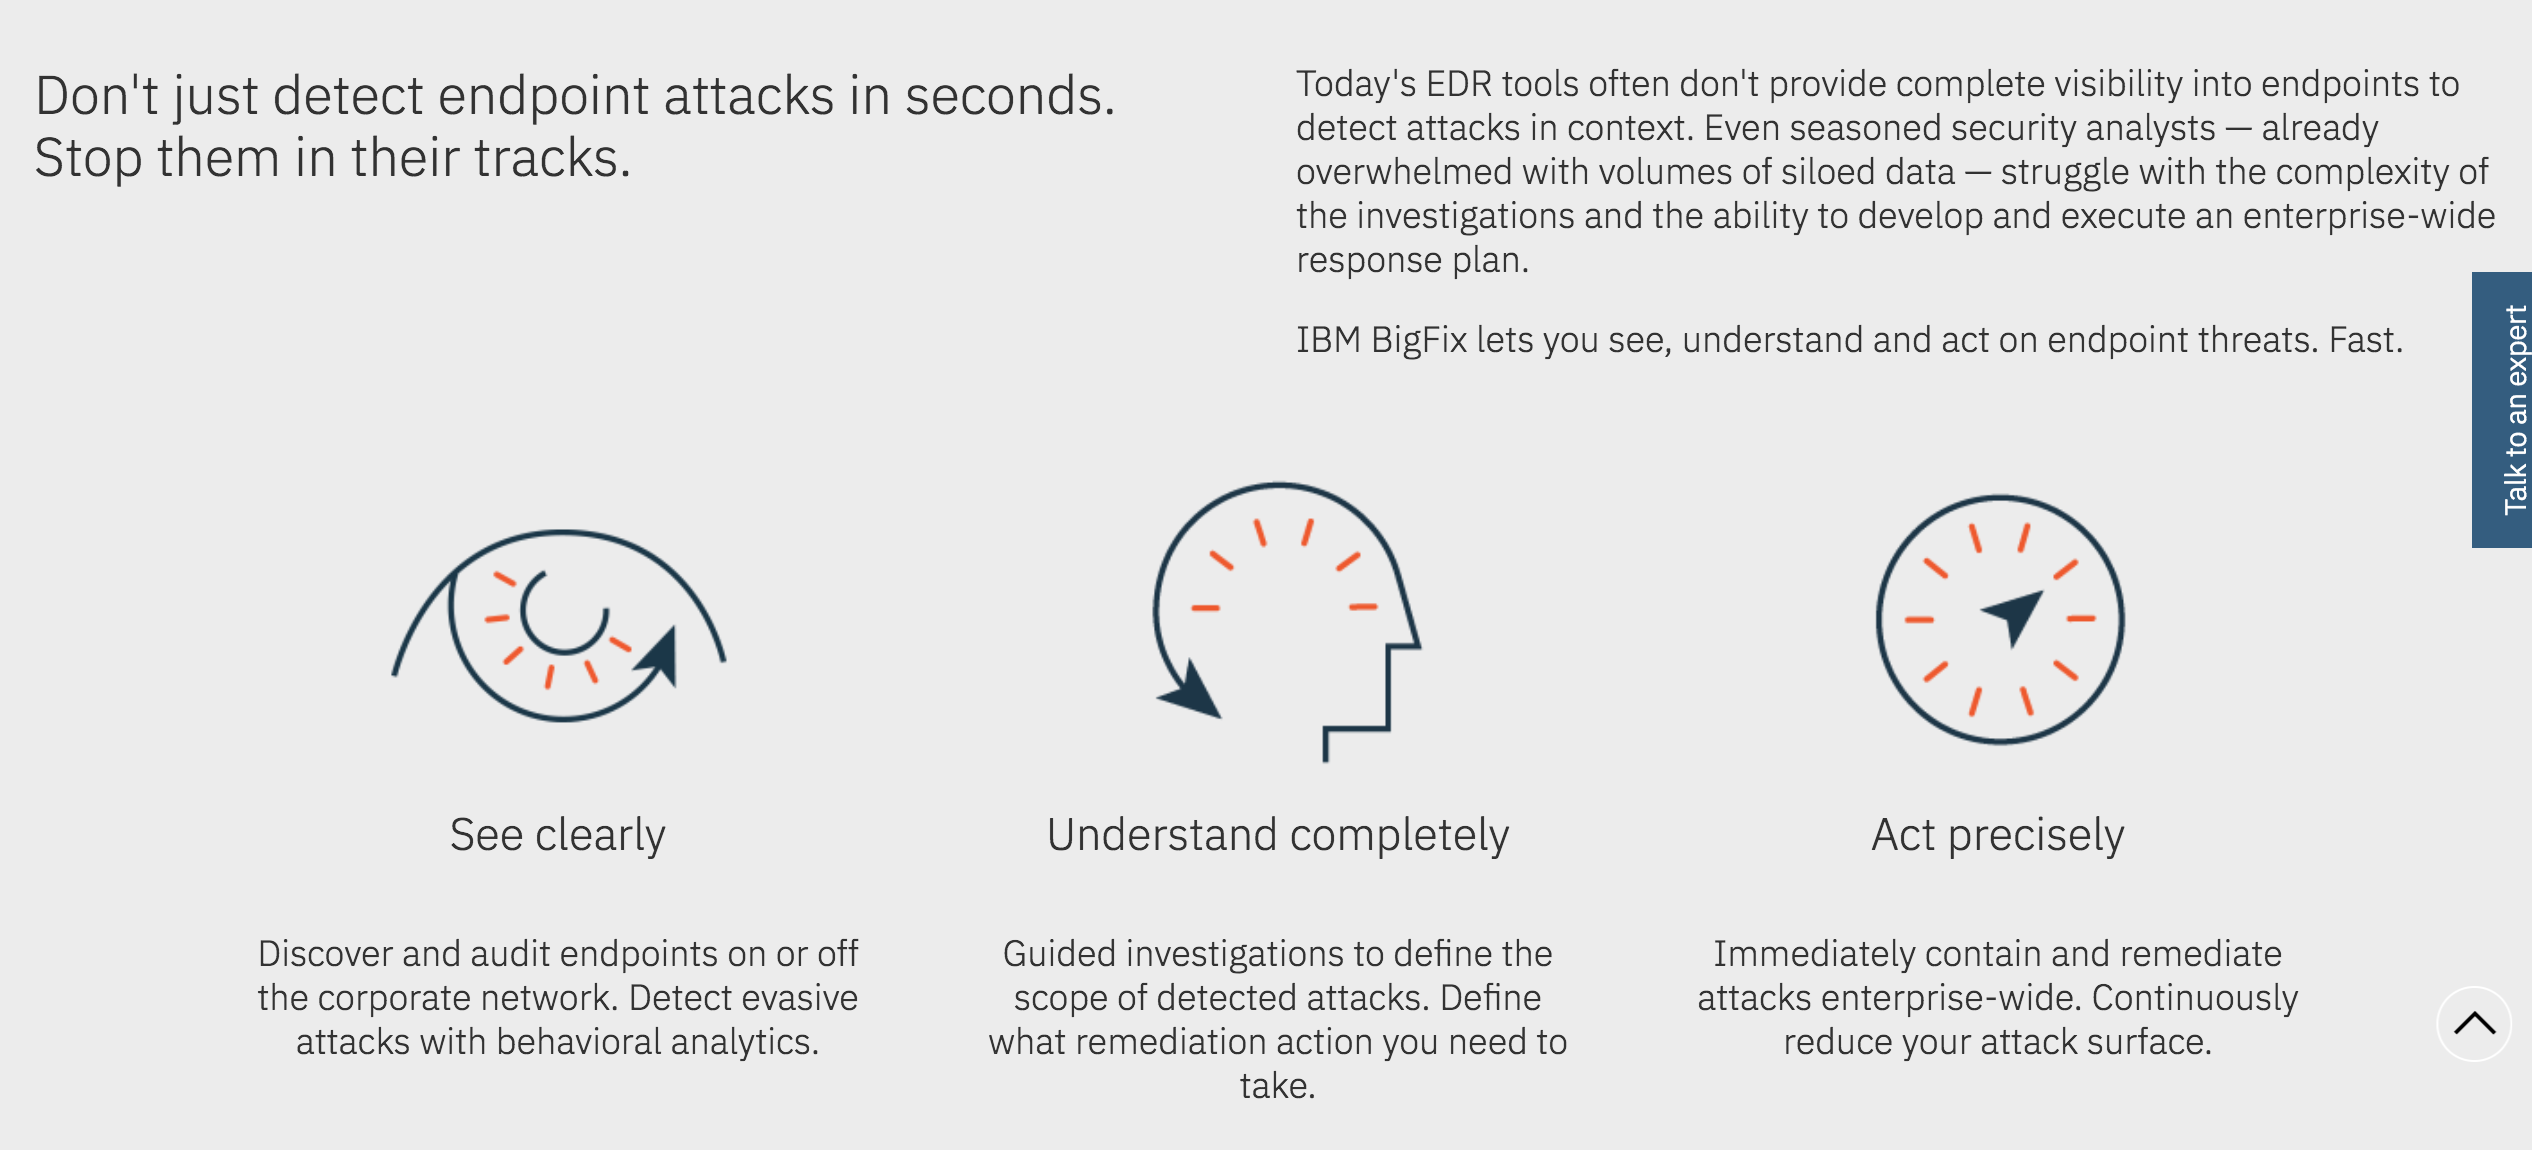
\includegraphics[width=\textwidth,keepaspectratio=true]{capitoli/imgs/BigFixManifest.png}
	\caption{Breve header descrittivo di BigFix dal sito web di IBM Security}
\end{figure}
\subsection{Architettura}
L'architettura di BigFix può essere, per sua natura, molto articolata, nel caso si debba gestire un numero elevato ed eterogeneo di dispositivi. Essa si basa sul consolidato pattern stilistico client/server, ma con una struttura leggermente variata, prevedendo l'inserimento di un ulteriore layer frapposto tra client e server, i Relay, i quali sono fondamentali per bilanciare il carico di lavoro.
\paragraph{}
Ma partiamo subito con un esempio per avere un ponto di riferimento.
\begin{figure}[h!]
	\centering
	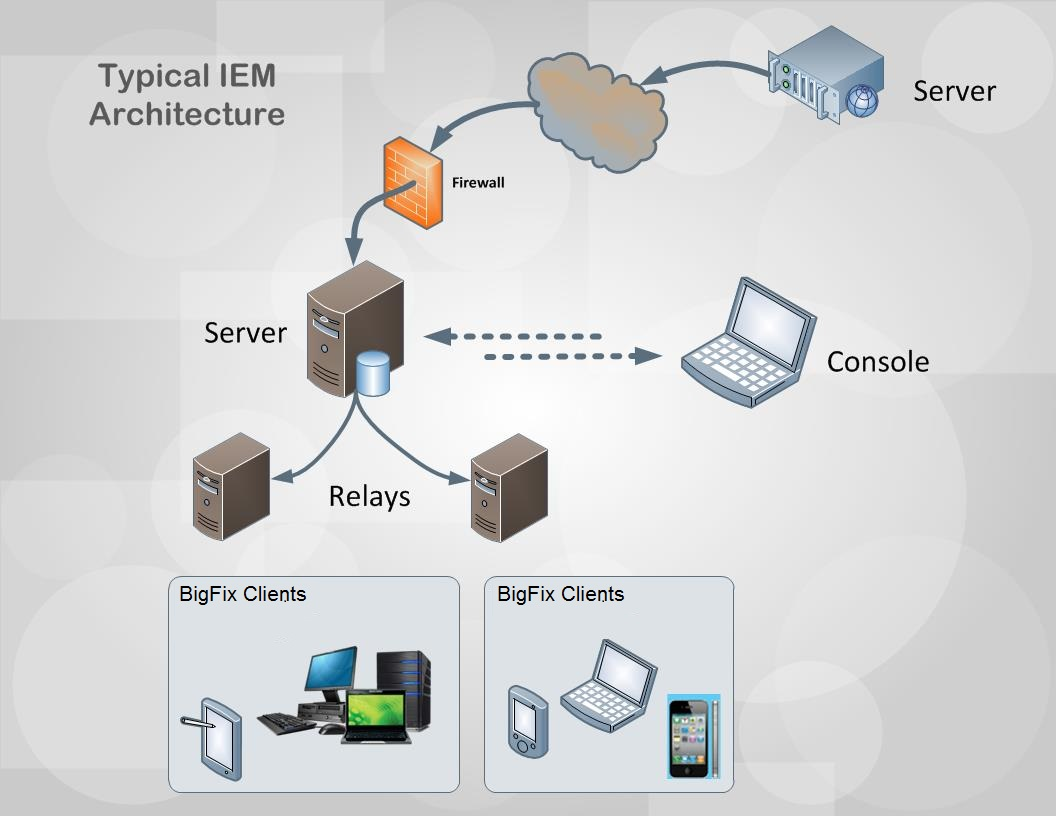
\includegraphics[width=\textwidth,keepaspectratio=true]{capitoli/imgs/IEMArchitecture.png}
	\caption{Un'architettura BigFix di esempio}
\end{figure}
Come possiamo notare, l'elemento centrale è il server di BigFix, il quale ha lo scopo di raccogliere dei particolari messaggi chiamati Fixlet. Questi messaggi dovono poi venire inoltrati ai Relay. E' competenza dei Relay interagire con i singoli client e assicurarsi che le Fixlet siano eseguite. Esse, infatti, altro non sono che delle azioni che devono essere necessariamente compiute dai dispositivi. Una sorta di "catalogo" delle Fixlet più utili può essere trovato sul Content server che è accessibile via internet dagli utenti. In tutto ciò la "finestra" dalla quale opera l'amministratore è ovviamente la Console, la quale monitora tutto il flusso di lavoro di BigFix. Andiamo ora ad analizzare le singole componenti dell'architettura.
\paragraph{Servers}
Il server coordina tutto il flusso di informazioni e si preoccupa di salvare le informazioni sul database. Al tempo stesso però, lascia agli Agent il compito di effettuare analisi ed eseguire azioni specifiche. Ciò consente di liberare il server da una pesantissima computazione. Per questo motivo esso può gestire un altissimo numero di client.
\paragraph{Relays}
I Relay si comportano come una cache tra i client e il server e sono di numero variabile in base al numero di client. Aiutano il server a gestire i dispositivi anche se funzionalmente non sono altro che client che sono stati promossi a Relay, aggiungendo a loro dei servizi. A questo punto i client non si interfacceranno mai con il server, alleggerendone così notevolmente il workload. Possono, ad esempio, più client richiedere un download al Relay, il quale effettuerà un'unica richiesta al server
\paragraph{Agents}
Un Agent è installato su ogni client facente parte dell'architettura di BigFix. Essi hanno il compito di raccogliere le Fixlet, tramite le quali sono in grado di compiere tutte le azioni necessarie. Un Agent fa dei continui controlli per confrontare lo stato del dispositivo con le policy stabilite. Appena scopre che il dispositivo è fuori dalla compliance, informa il server ed agisce subito per porre rimedio e, al termine dell'attività, l'Agent informa nuovamente il server sull'esito dell'operazione.
\paragraph{Web Reports}
I Web Reports costituiscono il componente che consente ad utenti autorizzati di monitorare tutti i dispositivi di BigFix. Si può, in questo modo, tenere traccia di vulnerabilità, azioni richieste e molto altro.
\paragraph{Consoles}
La Console permette agli amministratori di interagire con tutti i client dell'ambiente BigFix. Gli utenti possono così distribuire velocemente patch e configurazioni.
\paragraph{Content Server (BES SUpport)}
Il Content server è una sorta di repository. Contiene Fixlet a bassa personalizzazione che fanno fronte a esigenze più o meno comuni a tutti gli utenti BigFix. Possono essere prelevate ed utilizzati per i propri fini.
\paragraph{}
BigFix, da un punto di vista logico, si suddivide in due grandi macro-componenti, la Platform e le Applications. La prima svolge la funzione di layer sopra la quale vengono sviluppate tutte le funzionalità dello strato di applications. Questa organizzazione consente una chiara suddivisione delle competenze da parte di progettisti, sviluppatori, tester e assistenti dei clienti. Il team della Platform si concentra quindi nel fornire una solida infrastruttura al team delle Applications, il quale svilupperà i singoli strumenti al servizio dell'utente.
\subsection{BigFix Platform}
La Platform è una tecnologia multi-layer scritta in linguaggio C++ che agisce come colonna portante di tutta l'infrastruttura di BigFix. Essa svolge infatti funzioni fondamentali, spesso utilizzate anche da altre applicazioni dei layer superiori. Le attività della Platform sono fondamentali per la sussistenza dell'architettura che abbiamo descritto poco fa.

\subsection{BigFix Applications}
Tutti i prodotti applicativi che fanno parte di questo componente consentono di gestire in maniera semplice le operazioni inerenti alla security. A differenza della Platform, sono implementate in linguaggio Java o JavaScript ed hanno funzionalità atomiche tra di loro. Sono l'interfaccia principale con il quale interagisce l'amministratore aziendale.

\paragraph{BigFix Lifecycle}
Questa è l'applicazione che l'amministratore utilizza per gestire il ciclo di vita degli endpoint fisici. Ha una visibilità completa su di essi e pone rimedi immediati. Tra le funzioni principali ci sono quelle di power management, software distribution e OS deployment. 
\paragraph{BigFix Patch}
E' l'applicazione che consente la distribuzione di patch sia a livello di applicativi che a livello di sistema operativo.
\paragraph{BigFix Compliance}
Si utilizza questa applicazione per garantire la compliance dei dispositivi, identificare irregolarità e risolverle.
\paragraph{BigFix Protection}
Questa applicazione viene adoperata per garantire una protezione real-time contro qualsiasi genere di malware (virus, trojan, worms, spyware, rootkits e altre minacce web). Ha ovviamente effetto sia sugli endpoint fisici che sulle macchine virtuali.
\paragraph{BigFix Inventory}
Come dice la parola stessa, questa applicazione si occupa di analizzare gli endpoint e generare un inventario di tutti i software su essi installati, generando dei report ed evidenziando, eventualmente, le irregolarità.

\subsection{Fixlets}
Le Fixlet sono il metodo attraverso il quale si svolgono tutte le operazioni, come distribuzione di software, installazioni di patch e configurazioni. Esse sono dei messaggi inoltrati ai client di BigFix e utilizzano un linguaggio di query specifico, il Relevance.
\subsubsection{Il linguaggio Relevance}
Con una Fixlet si può anche ispezionare un desiderato aspetto di un client. A tale scopo viene adoperato il linguaggio Relevance. Esso, infatti, consente di interrogare il client, identificandone caratteristiche dell'hardware o del software tramite particolari costrutti, gli Inspectors. Una necessità può essere infatti quella di applicare una Fixlet solamente a dei client con determinate caratteristiche hardware/software oppure che si trovano in stati ben definiti. Si può, in questo modo, facilmente identificare il corretto sottoinsieme di client ai quali è destinata una nuova Fixlet ed applicarla solo ad essi.

\section{IBM}
Come detto, il lavoro di tesi si è svolto nell'ambito di un progetto formativo stipulato tra l'Università dell'Aquila e IBM Italia Spa. Questo progetto ha previsto un tirocinio svolto nella seda di Roma con obiettivo: "Esplorazione e prototipazione di metodi per portare prodotti BigFix su cloud", per l'appunto la realizzazione del prototipo di BigFix Saas. 
\paragraph{}
La storia dell'IBM ha inizio nei primi decenni del novecento, ma è dagli anni settanta che entra nel mercato dell'informatica, soprattutto nel settore hardware. Negli ultimi venti anni il business si è spostato sempre più sul software. In particolare soluzioni cognitive e piattaforme cloud.
\paragraph{IBM Security}
Presso la sede di Roma presente il più importante laboratorio IBM italiano, il Rome Software Lab. Nella divisione italiana ci si concentra prevalentemente sullo sviluppo back-end. Una grossa fetta del laboratorio fa parte della divisione Security di IBM. Il portfolio di Security contiene per l'appunto prodotti che si occupano di diversi aspetti della security aziendale, tra questi BigFix è uno dei più consolidati.

\section{SaaS Exploration Project}
Lo scopo del progetto al quale ho partecipato con il mio lavoro è quello di esplorare le tecnologie esistenti nel panorama cloud e realizzare il prototipo della versione SaaS di BigFix. A questo scopo, oltre a me, sono state allocate altre tre persone full time al conseguimento del progetto, sotto la guida dell'Architect Bernardo Pastorelli.

\subsection{Il framework SCRUM}
Il team adotta il framework agile SCRUM. Questo modo di operare è di sempre maggiore diffusione ed è basato su un approccio iterativo e incrementale nello sviluppo software. Il design e lo sviluppo sono divisi in iterazioni, denominate "Sprint", della durata fissa di due settimane. Queste due settimane terminano sempre con una versione funzionante del prodotto, il quale viene mostrato in una demo che evidenzia le nuove features implementate.
\paragraph{}
SCRUM utilizza un approccio empirico alla progettazione. La filosofia di fondo del framework è quella che la conoscenza deriva dall'esperienza, e quindi tutte le scelte che si prendono nel corso della progettazione devono avvenire alla luce di una sempre maggiore esperienza, la quale si ottiene avendo a disposizione il prima possibile un sottoinsieme del prodotto a se stante, testabile ed usabile. Dì qui l'approccio fortemente iterativo e incrementale massimizzando le opportunità di feedback. 
\paragraph{} 
All'inizio del progetto vengono definiti i requisiti del prodotto (item), i quali vengono da un'attenta analisi dei bisogni dell'utente. Ogni bisogno viene modellato con una Epica, che a sua volta viene prioritizzata e aggiunta al Product Backlog che le indicizza. Le Epiche vengono poi scomposte in User Stories, le quali si suddividono a loro volta in Task, ossia l'elemento atomico del progetto la cui implementazione viene presa in carico da un singolo componente del team.
\paragraph{}
L'inizio di uno Sprint è sempre caratterizzato da un meeting in cui si pianificano gli obiettivi. In questo contesto si fa sempre riferimento al Backlog incentrandosi sulle User Stories ancora non coperte. Si cerca quindi di suddividersi i Task in modo tale da avere a fine Sprint quelle nuove funzionalità usabili e dimostrabili. Demo che viene svolta sempre con la presenza di tutto il team e anche di colleghi di altri laboratori IBM.
\subsection{Sistemi di controllo di versione}
Da un'organizzazione di questo tipo ne scaturisce la necessità di tool di controllo di versione che permettano una fluida gestione del codice e della programmazione in parallelo tra i diversi componenti del team.
\paragraph{GitLab}
A tal scopo si è adottato ormai da tempo, da tutto il team di BigFix, il software di controllo di gestione distribuito Git e una repository aziendale che consiste in una versione enterprise ad hoc per IBM di GitLab, un hosting service molto simile a GitHub. 
\begin{figure}[h!]
	\centering
	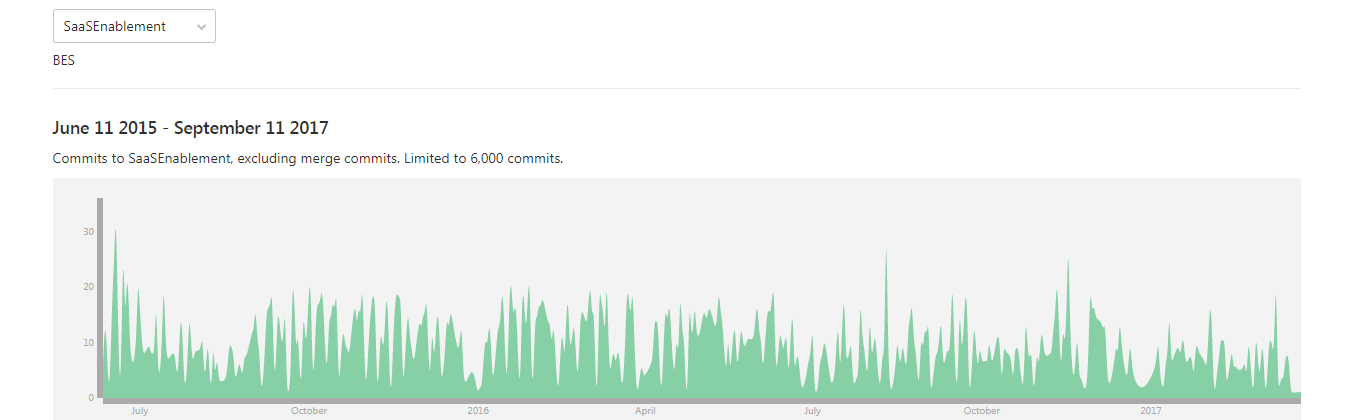
\includegraphics[width=\textwidth,keepaspectratio=true]{capitoli/imgs/GitLabGraph.PNG}
	\caption{Panoramica degli ultimi contributi nel branch del progetto SaaS}
\end{figure}
\paragraph{}
Il flusso di lavoro è il seguente. Quando inizia il proprio task, il componente del team si pone su un proprio branch personale sul quale effettua i propri commit. Al termine del task viene fatta una merge request sul branch principale, solo una volta che si è testato il codice, per aggiungere i propri contributi al progetto. A questo punto, dopo una review effettuata da componenti del team accreditati, il nuovo branch verrà mergiato con il branch principale.
\subsection{RTC}
E' ovviamente necessario un tool che coordini anche la suddivisione dei task all'interno del team. A tal fine abbiamo utilizzato un software di IBM, ovvero Rational Team Concert (RTC), il quale è disponibile anche esternamente e gratuito nel caso di piccoli team. Esso offre comodi strumenti di agile planning e gestione di ciclo di vita del software. Ogni componente del team può così tracciare facilmente le aree di sua competenza. E' possibile inoltre usufruire di tool per il source control, controllo dei difetti e gestione delle build.
\begin{figure}[h]
	\centering
	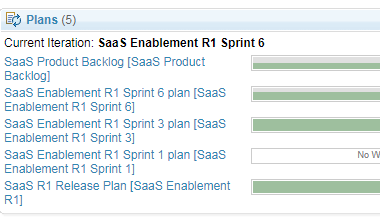
\includegraphics[width=0.5\linewidth]{capitoli/imgs/rtc2}
	\caption{RTC. Un'esempio di come viene monitorato il completamento dei diversi sprint}
	\label{fig:rtc2}
\end{figure}



